\chapter{Number Representation and Arithmetic Circuits}\label{ch:arith}

\begin{objectives}
After studying this chapter you will be able to:
\begin{itemize}
  \item convert numbers among decimal, binary, octal and hexadecimal;
  \item represent signed integers in sign-magnitude, one's-complement and two's-complement form, and explain why two's complement is used in practice;
  \item add and subtract two's-complement numbers and detect arithmetic overflow;
  \item design half adders, full adders, ripple-carry adders and adder/subtractor circuits, and describe them in VHDL;
  \item explain the delay problem of the ripple-carry adder and design a carry-lookahead adder using generate and propagate signals;
  \item multiply unsigned numbers with an array multiplier;
  \item represent fractions in fixed-point and IEEE~754 floating-point formats, and decimal digits and characters in BCD and ASCII.
\end{itemize}
\end{objectives}

\section{Positional Number Systems}\label{sec:numsys}
Section~\ref{sec:adc} showed that a binary string can represent a quantity. In a positional system with radix $r$ the value of the digit string $d_{n-1}\cdots d_1d_0.\,d_{-1}d_{-2}\cdots$ is $\sum_i d_i r^{\,i}$, with negative $i$ for the fraction. Four radices matter in digital design:
\begin{itemize}
  \item \textbf{Binary} ($r=2$), digits 0 and 1; each digit is a \term{bit}, and a group of eight bits is a \term{byte}.
  \item \textbf{Octal} ($r=8$), digits 0--7; one octal digit stands for exactly three bits.
  \item \textbf{Decimal} ($r=10$), the system used by people.
  \item \textbf{Hexadecimal} ($r=16$), digits 0--9 and A--F (A$=10$, \dots, F$=15$); one hex digit stands for exactly four bits. It is the usual compact way of writing binary values.
\end{itemize}
\Cref{tab:radix} lists the first values. The binary--octal--hex conversions are trivial because $8=2^3$ and $16=2^4$: group the bits in threes or fours starting at the binary point, and replace each group by its digit.

\begin{table}[htbp]
\centering
\small
\caption{The numbers 0 to 16 in four radices.}
\label{tab:radix}
\begin{tabular}{@{}cccc@{\hspace{2.5em}}cccc@{}}
\toprule
Dec & Binary & Oct & Hex & Dec & Binary & Oct & Hex\\
\midrule
0&00000&00&0 & 9 &01001&11&9\\
1&00001&01&1 & 10&01010&12&A\\
2&00010&02&2 & 11&01011&13&B\\
3&00011&03&3 & 12&01100&14&C\\
4&00100&04&4 & 13&01101&15&D\\
5&00101&05&5 & 14&01110&16&E\\
6&00110&06&6 & 15&01111&17&F\\
7&00111&07&7 & 16&10000&20&10\\
8&01000&10&8 & &&&\\
\bottomrule
\end{tabular}
\end{table}

\subsection{Converting from decimal}
To convert the \emph{integer part} to radix $r$, divide repeatedly by $r$ and collect the remainders; the first remainder is the least significant digit. To convert the \emph{fractional part}, multiply repeatedly by $r$ and collect the integer parts; the first is the most significant fractional digit.

\begin{example}{Radix conversion}{radix}
Convert $156_{10}$ to binary, hexadecimal and octal, and convert $0.6875_{10}$ to binary.

\textbf{Solution.} Dividing 156 by 2 repeatedly gives remainders $0,0,1,1,1,0,0,1$ (least significant first), so $156 = \bin{10011100}_2$. Grouping in fours gives $\bin{1001}\,\bin{1100}=9\mathrm{C}_{16}$, and grouping in threes ($\bin{010}\,\bin{011}\,\bin{100}$) gives $234_8$. Check: $2\cdot64+3\cdot8+4=156$.
For the fraction: $0.6875\times2=1.375\to1$; $0.375\times2=0.75\to0$; $0.75\times2=1.5\to1$; $0.5\times2=1.0\to1$, so $0.6875=\bin{0.1011}_2$.
\end{example}

\section{Signed Integer Representations}\label{sec:signed}
To represent negative numbers in binary, the most significant bit (MSB) is used as a \term{sign bit}: 0 means positive and 1 means negative (\cref{fig:msb}). Three schemes differ in how the remaining bits represent a negative value.

\figw{213.3pt}{lect_4_8bit_msb_lsb}{An 8-bit signed number: the MSB is the sign bit, the LSB is bit 0.}{fig:msb}

\paragraph{Sign-magnitude.} The remaining $n-1$ bits hold the magnitude. The range is $\pm(2^{n-1}-1)$ and there are \emph{two zeros}, $\bin{0000}$ ($+0$) and $\bin{1000}$ ($-0$). Arithmetic is awkward, since the signs and magnitudes must be compared first.

\paragraph{One's complement.} Positive numbers are as in sign-magnitude; a negative number is obtained by \emph{inverting every bit} of the positive number: $+5=\bin{0101}$, $-5=\bin{1010}$. There are again two zeros ($\bin{0000}$ and $\bin{1111}$). Addition requires an \emph{end-around carry}: the carry out of the MSB is added back to the result.

\paragraph{Two's complement.} A negative number is obtained by inverting all bits and \emph{adding 1}: $+5=\bin{0101}\to\bin{1010}\to\bin{1011}=-5$. There is only one zero, and the range is asymmetric: $-2^{n-1}$ to $2^{n-1}-1$. The value of an $n$-bit two's-complement number is
\begin{equation}
  V = -d_{n-1}\,2^{\,n-1} + \sum_{i=0}^{n-2} d_i\,2^{\,i}.
  \label{eq:twos}
\end{equation}
Hence $\bin{10110101} = -128+32+16+4+1=-75$. \Cref{tab:signed} compares the three schemes for 4-bit numbers.

\begin{table}[htbp]
\centering
\small
\caption{Four-bit signed numbers in the three representations.}
\label{tab:signed}
\begin{tabular}{@{}rccc@{\hspace{3em}}rccc@{}}
\toprule
Dec & Sign-mag. & 1's comp. & 2's comp. & Dec & Sign-mag. & 1's comp. & 2's comp.\\
\midrule
$+7$&0111&0111&0111 & $-0$&1000&1111&---\\
$+6$&0110&0110&0110 & $-1$&1001&1110&1111\\
$+5$&0101&0101&0101 & $-2$&1010&1101&1110\\
$+4$&0100&0100&0100 & $-3$&1011&1100&1101\\
$+3$&0011&0011&0011 & $-4$&1100&1011&1100\\
$+2$&0010&0010&0010 & $-5$&1101&1010&1011\\
$+1$&0001&0001&0001 & $-6$&1110&1001&1010\\
$+0$&0000&0000&0000 & $-7$&1111&1000&1001\\
    &&&              & $-8$&---&---&1000\\
\bottomrule
\end{tabular}
\end{table}

\begin{example}{Two's-complement conversions}{twos}
(a)~Represent $-75$ as an 8-bit two's-complement number, in binary and hexadecimal. (b)~Find the decimal value of $\bin{1011\,0101}$. (c)~Extend $\bin{1011}$ ($-5$) to 8 bits.

\textbf{Solution.} (a)~$+75=\bin{0100\,1011}$. Invert: $\bin{1011\,0100}$. Add 1: $\bin{1011\,0101}=\mathrm{B5}_{16}$. (b)~Using \cref{eq:twos}, $-128+32+16+4+1=-75$; this is indeed the number found in~(a). (c)~To widen a two's-complement number, \term{sign-extend} it by copying the sign bit into the new upper bits: $\bin{1111\,1011}$, which is again $-5$ ($-128+64+32+16+8+2+1=-5$).
\end{example}

\begin{keypoint}[Why two's complement?]
Two's complement has a single zero, a simple negation (invert and add 1), and, above all, \emph{the same adder circuit adds signed and unsigned numbers}: subtraction is just addition of the negated operand. This is why every modern processor uses it.
\end{keypoint}

\section{Arithmetic and Overflow}\label{sec:overflow}
\Cref{ex:addrep} shows the calculation $4+(-3)$ in the three representations.

\begin{example}{$4+(-3)$ in the three systems}{addrep}
\textbf{Sign-magnitude.} $+4=\bin{0100}$, $-3=\bin{1011}$. The signs differ, so subtract the smaller magnitude from the larger: $\bin{100}-\bin{011}=\bin{001}$, with the sign of the larger magnitude (positive): $\bin{0001}=+1$.\\
\textbf{One's complement.} $-3=\bin{1100}$. $\bin{0100}+\bin{1100}=\bin{1\,0000}$. The end-around carry gives $\bin{0000}+1=\bin{0001}=+1$.\\
\textbf{Two's complement.} $-3=\bin{1101}$. $\bin{0100}+\bin{1101}=\bin{1\,0001}$. Discarding the carry-out gives $\bin{0001}=+1$.
\end{example}

If the true result of an operation lies outside the range of the representation, \term{arithmetic overflow} occurs and the result is wrong. With $n$ bits the range for signed numbers is $-2^{n-1}$ to $2^{n-1}-1$. For example, in 4 bits $(+7)+(+2)=+9$ computes as $\bin{0111}+\bin{0010}=\bin{1001}$, which reads as $-7$. Similarly $(-7)+(-2)=\bin{1001}+\bin{1110}=\bin{1\,0111}$, which after discarding the carry reads as $+7$. Two facts make detection easy. First, overflow \emph{cannot occur when the operands have different signs}. Second, when it does occur, the carry into the sign bit differs from the carry out of it.

\begin{keypoint}[Overflow rule for two's complement]
Let $c_{n-1}$ be the carry into the sign-bit position and $c_n$ the carry out of it. Overflow occurs if and only if
\[
  \text{overflow} = c_{n-1}\xor c_n .
\]
\end{keypoint}

In the first example, $c_4=0$ and $c_3=1$; in the second, $c_4=1$ and $c_3=0$. In both cases the two carries differ, so overflow is signalled.

\section{Adders}\label{sec:adders}
\subsection{Half adder and full adder}
The half adder of \cref{ex:half-adder} adds two bits. To add multi-bit numbers we need to include the carry arriving from the lower position: a \term{full adder} (FA) adds three bits, $A$, $B$ and $C_{in}$, and produces a sum $S$ and carry-out $C_{out}$ (\cref{tab:fa}). From the truth table
\begin{equation}
 S = A\xor B\xor C_{in}, \qquad C_{out} = AB + C_{in}(A\xor B).
 \label{eq:fa}
\end{equation}
The carry output is the \emph{majority} function of the three inputs, so it also equals $AB + AC_{in} + BC_{in}$.

\begin{table}[htbp]
\centering
\caption{Truth table of the full adder.}
\label{tab:fa}
\begin{tabular}{ccc|cc}
\toprule
$A$&$B$&$C_{in}$&$C_{out}$&$S$\\ \midrule
0&0&0&0&0\\0&0&1&0&1\\0&1&0&0&1\\0&1&1&1&0\\
1&0&0&0&1\\1&0&1&1&0\\1&1&0&1&0\\1&1&1&1&1\\ \bottomrule
\end{tabular}
\end{table}

Equation~\eqref{eq:fa} shows that a full adder can be built from \emph{two half adders and an OR gate}: the first half adder adds $A$ and $B$ giving $S_1=A\xor B$ and $C_1=AB$; the second adds $S_1$ and $C_{in}$ giving $S=S_1\xor C_{in}$ and $C_2=S_1C_{in}$; and $C_{out}=C_1+C_2$ (\cref{fig:fa}). \Cref{lst:fa} is the corresponding \emph{structural} VHDL description, in which a design is written as a set of component instances connected by signals; it uses the half-adder entity of \cref{lst:half-adder}.

\begin{figure}[htbp]
\centering
\begin{subfigure}[b]{324.2pt}\centering
  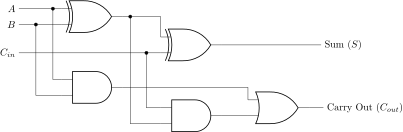
\includegraphics[width=322.2pt]{lect_4_circuit_full_adder}\caption{gate-level circuit}
\end{subfigure}
\\[6pt]
\begin{subfigure}[b]{299.2pt}\centering
  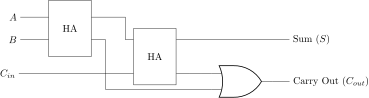
\includegraphics[width=297.2pt]{lect_4_circuit_full_adder_from_ha}\caption{from two half adders}
\end{subfigure}
\caption{Two implementations of the full adder.}\label{fig:fa}
\end{figure}

\vhdlfile[firstline=1, lastline=57]{../vhdl/full_adder.vhd}{Structural VHDL of the full adder, built from two half-adder components.}{lst:fa}

\subsection{Ripple-carry adder}
To add two $n$-bit numbers we cascade $n$ full adders: the carry-out of stage $i$ becomes the carry-in of stage $i+1$. The first carry-in $C_0$ is 0 for ordinary addition. \Cref{fig:ripple} shows a 4-bit \term{ripple-carry adder}, so called because the carry ``ripples'' from the least significant to the most significant stage. \Cref{lst:ripple} describes it in VHDL using a \code{std_logic_vector}, which is an array of bits written with an index range such as \code{(3 downto 0)}, and an internal vector of carries.

\figw{301.8pt}{lect_4_circuit_ripple_adder}{A 4-bit ripple-carry adder built from four full adders.}{fig:ripple}

\vhdlfile{../vhdl/ripple_adder_4bit.vhd}{Structural VHDL of a 4-bit ripple-carry adder.}{lst:ripple}

\Cref{fig:sim-ra} shows a ModelSim simulation of this adder using a testbench with assertions: $0+0$, $1+1$, $15+1$ (carry out, sum $0000$), $15+15+1$ (sum $1111$, carry out 1) and $5+3$ (sum $1000$). The testbenches of this chapter, in the style of \cref{lst:tb}, are provided with the book's source files.

\begin{figure}[htbp]
\centering
\wavesplit{lect_4_sim_result_RA}{3}\vspace{4pt}
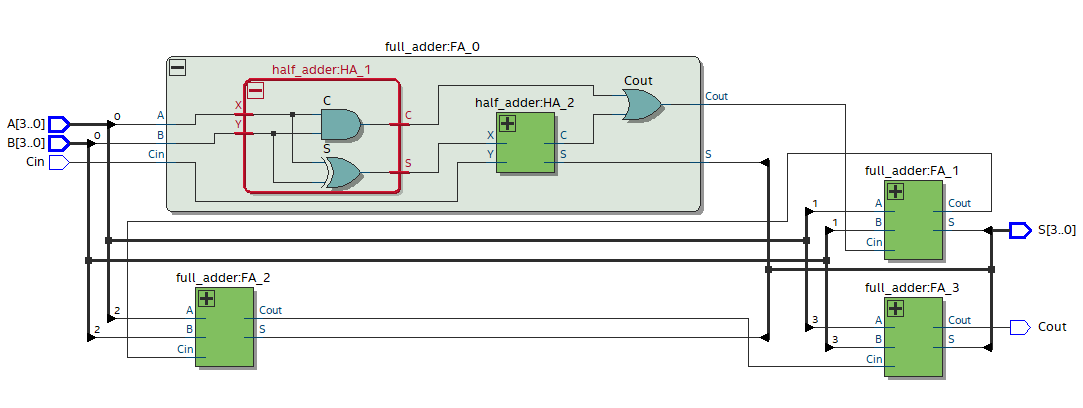
\includegraphics[width=\linewidth]{lect_4_rtl_viewer_RA}
\caption{Ripple-carry adder: ModelSim simulation of the testbench (top) and the RTL viewer schematic produced by Quartus (bottom), author's screenshots.}
\label{fig:sim-ra}
\end{figure}

\subsection{Adder/subtractor}
Since $A-B = A+(-B) = A+\NOT{B}+1$ in two's complement, the same adder performs subtraction if the bits of $B$ are inverted and the initial carry-in is 1. An XOR gate works as a \emph{controllable inverter}: $B_i\xor 0=B_i$ and $B_i\xor 1=B_i'$. With a control input $\mathit{sub}$ ($0$ = add, $1$ = subtract) connected both to the XOR gates and to $C_0$ we obtain the adder/subtractor of \cref{fig:addsub}. When $\mathit{sub}=0$ the circuit computes $A+B$, and when $\mathit{sub}=1$ it computes $A+\NOT{B}+1=A-B$. The overflow signal is $c_{n-1}\xor c_n$.

\figw{245.5pt}{lect_4_circuit_adder_subtractor}{A 4-bit adder/subtractor. The XOR gates conditionally complement $B$, and the control input is also the initial carry.}{fig:addsub}

\vhdlfile{../vhdl/adder_subtractor_4bit.vhd}{VHDL of the 4-bit adder/subtractor, reusing the ripple-carry adder.}{lst:addsub}

\begin{figure}[htbp]
\centering
\wavesplit{lect_4_sim_result_AS}{4}
\caption{ModelSim simulation of the adder/subtractor: $5+3=8$, $5-3=2$, $3-5=-2$ ($\bin{1110}$), $7+2$ (overflow, $\bin{1001}$) and $-8-1$ (overflow, $\bin{0111}$). Author's screenshot.}
\label{fig:sim-as}
\end{figure}

\section{The Carry Delay and the Carry-Lookahead Adder}\label{sec:cla}
\subsection{Delay of the ripple-carry adder}
The \term{critical path}, the longest delay between an input change and a stable output, of a ripple-carry adder passes through the carry chain. The worst case, for example $\bin{1111}+\bin{0001}$, requires the carry generated in the first stage to travel through every later stage. If each full adder adds two gate delays on the carry path, an $n$-bit adder has a delay of about $2n$ gate delays, so a 16-bit adder needs about $32$ gate delays (\cref{fig:rcdelay}). The delay grows linearly with $n$, which is unacceptable in a fast processor.

\figw{353.1pt}{lect_4_ripple_carry_delay}{The carry must ripple through every stage in the worst case.}{fig:rcdelay}

\subsection{Generate and propagate}
A \term{carry-lookahead adder} (CLA) computes all the carries in parallel directly from the inputs, which removes the long dependency chain. The key is to re-express the full adder in terms of two signals for each bit position $i$:
\begin{itemize}
  \item the \term{generate} signal $G_i = A_iB_i$: stage $i$ produces a carry by itself, regardless of its carry-in;
  \item the \term{propagate} signal $P_i = A_i\xor B_i$: stage $i$ passes its carry-in on to its carry-out.
\end{itemize}
Then
\begin{equation}
  S_i = P_i\xor C_i, \qquad C_{i+1} = G_i + P_iC_i .
  \label{eq:gp}
\end{equation}
Substituting repeatedly removes the dependence on the previous carry:
\begin{align*}
 C_1 &= G_0 + P_0C_0,\\
 C_2 &= G_1 + P_1G_0 + P_1P_0C_0,\\
 C_3 &= G_2 + P_2G_1 + P_2P_1G_0 + P_2P_1P_0C_0,\\
 C_4 &= G_3 + P_3G_2 + P_3P_2G_1 + P_3P_2P_1G_0 + P_3P_2P_1P_0C_0 .
\end{align*}
Each carry is a two-level AND--OR expression of the $P_i$, $G_i$ and $C_0$ only, and all four are computed at the same time (\cref{fig:cla4}).

\figw{364.8pt}{lect_4_circuit_cla_4bit}{Block diagram of a 4-bit carry-lookahead adder: a P/G generator for each bit, the lookahead logic, and sum XOR gates.}{fig:cla4}

\Cref{lst:cla-logic} is the lookahead logic block in VHDL and \cref{lst:cla4} is the top-level design, which instantiates the P/G units, the lookahead block and the sum gates.

\vhdlfile{../vhdl/cla_logic.vhd}{Carry-lookahead logic block of the 4-bit CLA.}{lst:cla-logic}

\vhdlfile{../vhdl/cla_4bit_adder.vhd}{Top level of the 4-bit carry-lookahead adder.}{lst:cla4}

\subsection{Hierarchical lookahead}
The fan-in (number of inputs) of the gates in a lookahead circuit grows with the word length, so a single-level CLA is impractical for 16 or 32 bits. The remedy is to build a \emph{hierarchy}: a 16-bit adder is made of four 4-bit CLA blocks, and a second-level lookahead unit computes the carries between the blocks. Each 4-bit block supplies a block-propagate and a block-generate signal:
\begin{align*}
 P^*_0 &= P_3P_2P_1P_0, & G^*_0 &= G_3 + P_3G_2 + P_3P_2G_1 + P_3P_2P_1G_0,
\end{align*}
and similarly $P^*_1,G^*_1$ for bits 4--7, $P^*_2,G^*_2$ for bits 8--11 and $P^*_3,G^*_3$ for bits 12--15. The block carries follow the same pattern as the bit carries:
\begin{align*}
 c_4 &= G^*_0 + P^*_0c_0,\\
 c_8 &= G^*_1 + P^*_1G^*_0 + P^*_1P^*_0c_0,\\
 c_{12} &= G^*_2 + P^*_2G^*_1 + P^*_2P^*_1G^*_0 + P^*_2P^*_1P^*_0c_0 .
\end{align*}
The structure is shown in \cref{fig:cla16}.

\figside{501.5pt}{lect_4_16-bit_cla}{A 16-bit adder with four 4-bit carry-lookahead blocks and a second-level lookahead unit.}{fig:cla16}

\begin{example}{Delay comparison for 16 bits}{cladelay}
Take one gate delay as $t$.

\textbf{Ripple-carry:} the carry passes through 16 full adders at $2t$ each: $16\times2t=32t$.

\textbf{Hierarchical CLA:} (1)~all $P_i$ and $G_i$: $1t$; (2)~block $P^*$ and $G^*$: $2t$; (3)~second-level lookahead gives $c_4,c_8,c_{12}$: $2t$; (4)~the carries inside each block: $2t$; (5)~the sum bits $S_i=P_i\xor C_i$: $1t$. The total is $1+2+2+2+1 = 8t$, four times faster than the ripple-carry adder, at the price of more gates.
\end{example}

\begin{figure}[htbp]
\centering
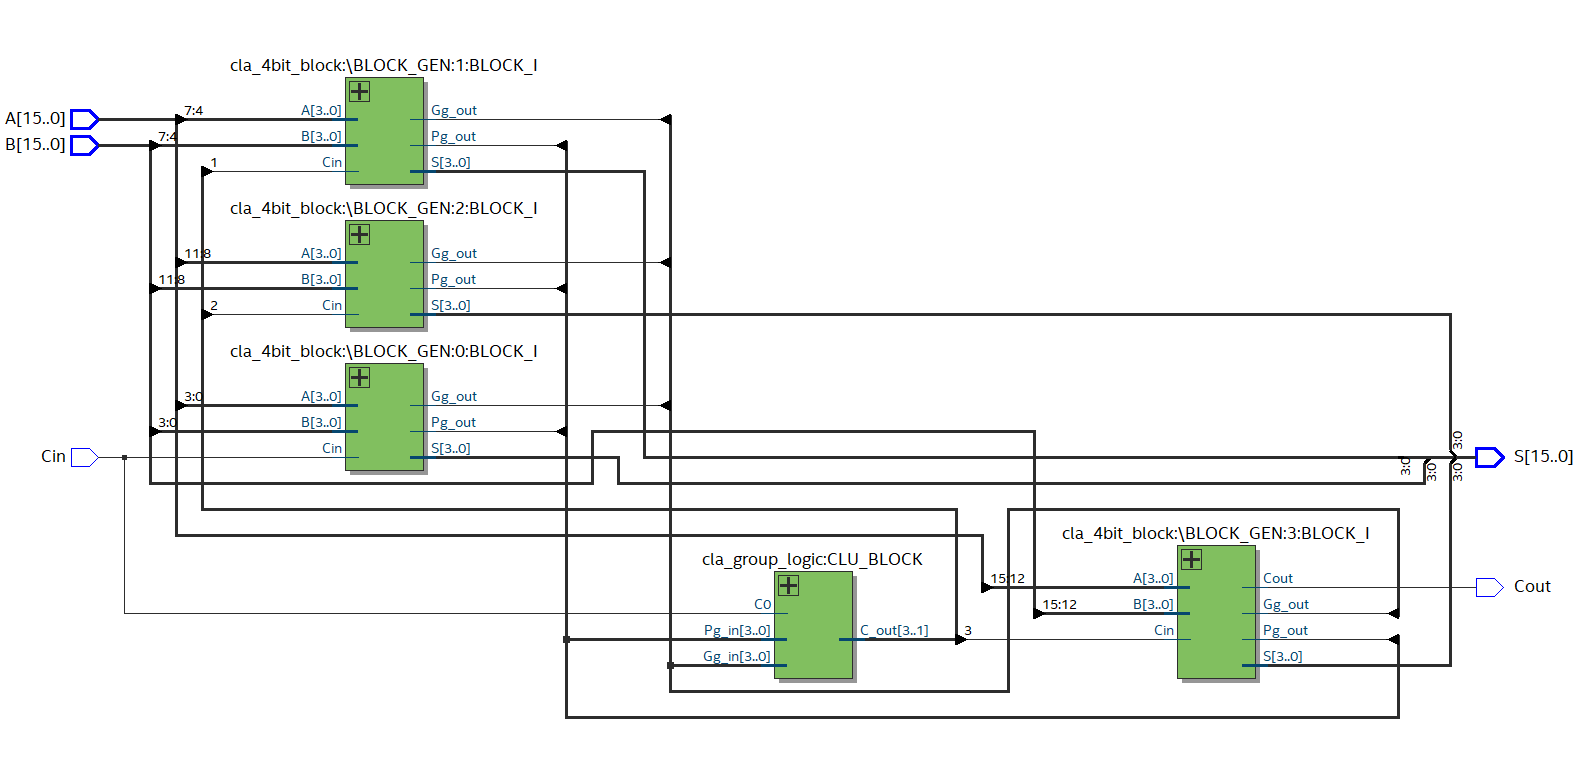
\includegraphics[width=\linewidth]{lect_4_rtl_viewer_cla_16bit}\\[4pt]
\wavesplit{lect_4_sim_result_cla_16bit}{3}
\caption{16-bit carry-lookahead adder: RTL viewer (top) and ModelSim simulation (bottom). Author's screenshots. The VHDL files \code{cla_4bit_block}, \code{cla_group_logic} and \code{cla_16bit_adder} accompany the book.}
\label{fig:cla16-sim}
\end{figure}

\section{Multiplication}\label{sec:mult}
Binary multiplication is a process of adding \emph{partial products}. Because each multiplier bit is 0 or 1, each partial product is either zero or a copy of the multiplicand, shifted to the position of the multiplier bit.

\begin{example}{Multiplying $1101\times1011$}{mult}
Multiply $A=\bin{1101}\ (13)$ by $B=\bin{1011}\ (11)$.
\begin{center}\ttfamily
\begin{tabular}{@{}r@{}}
\phantom{000}1101\\
$\times$\ \ 1011\\ \hline
\phantom{000}1101\\
\phantom{00}11010\\
\phantom{0}000000\\
1101000\\ \hline
10001111
\end{tabular}
\end{center}
The partial products are $A\times B_0$, $A\times B_1$ (shifted one place), and so on; adding them, $\bin{1101}+\bin{11010}+\bin{000000}+\bin{1101000}=13+26+0+104=143=\bin{10001111}$. The product of two 4-bit numbers needs up to 8 bits.
\end{example}

An \term{array multiplier} implements this directly. An AND gate forms each bit of the partial products, $A_iB_j$, and an array of adders adds them with the correct shifts. For a $4\times4$ multiplier (\cref{fig:mult4}) we need 16 AND gates and 12 adders (3 half adders and 9 full adders in the design of \cref{lst:mult}). \Cref{lst:mult} also shows the VHDL \code{generate} statement, which replicates hardware: here it creates the 16 AND gates.

\figw{410.0pt}{lect_4_multiplier_4x4}{A $4\times4$ array multiplier: partial products are formed by AND gates and summed by rows of adders.}{fig:mult4}

\vhdlfile[firstline=1, lastline=62]{../vhdl/multiplier_4x4.vhd}{VHDL of the $4\times4$ array multiplier (first part: declarations, partial products and the first adder row). The remaining rows follow the same pattern.}{lst:mult}

\begin{figure}[htbp]
\centering
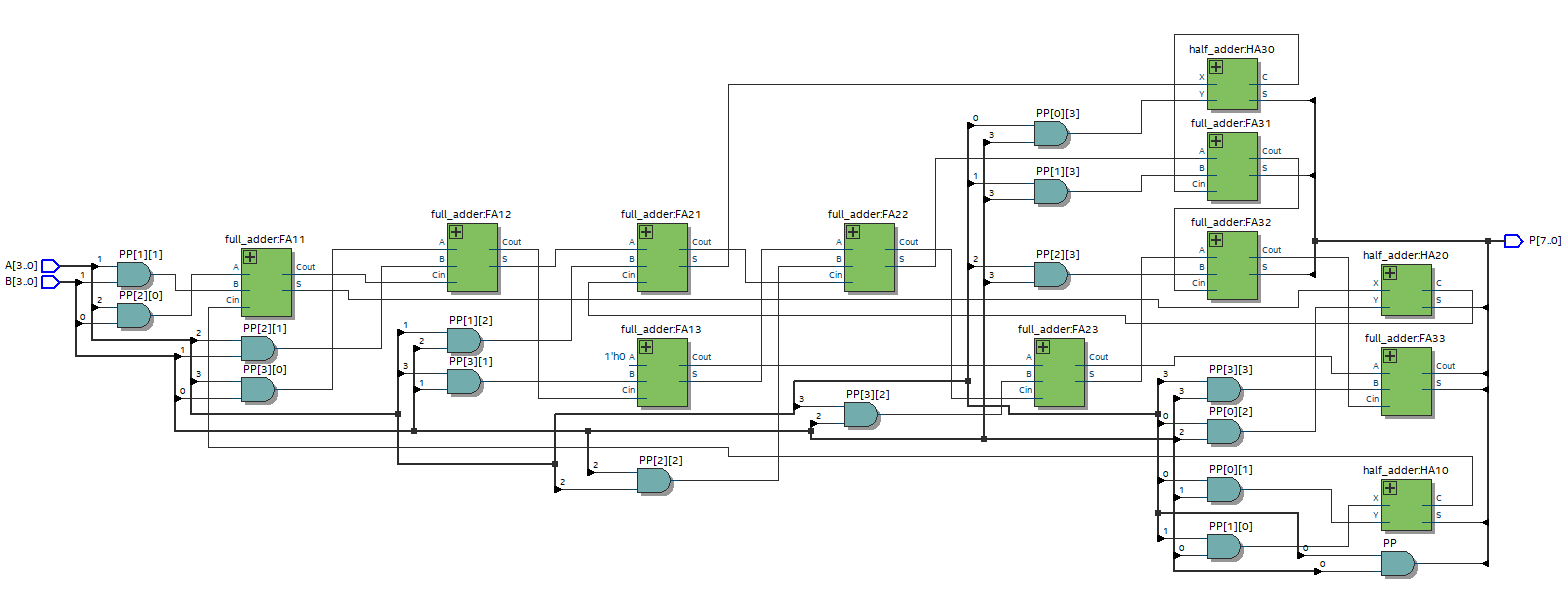
\includegraphics[width=\linewidth]{lect_4_rtl_viewer_mul_4x4}\\[4pt]
\wavesplit{lect_4_sim_result_mul_4x4}{3}
\caption{$4\times4$ multiplier: RTL viewer (top) and ModelSim simulation (bottom). Author's screenshots.}
\label{fig:mult-sim}
\end{figure}

\section{Fractions and Floating Point}\label{sec:fixfloat}
\subsection{Fixed-point numbers}
A \term{fixed-point} number represents a fraction with a fixed number of bits for the integer and fractional parts; the binary point is implicit. The notation $Qn.m$ means $n$ integer bits and $m$ fractional bits (unsigned unless stated otherwise); the resolution is $2^{-m}$ and the range $0$ to $2^n-2^{-m}$. Fixed-point arithmetic uses ordinary integer hardware, so it is fast, small and low-power, but the range and precision are limited and the designer must choose the format carefully to avoid overflow and loss of precision.

\begin{example}{Fixed-point conversion}{fixed}
Represent $6.75_{10}$ in $Q4.4$ format (8 bits).

\textbf{Solution.} The integer part is $6=\bin{0110}$. The fraction: $0.75\times2=1.5\to1$; $0.5\times2=1.0\to1$; then $0, 0$. So $0.75=\bin{.1100}$ and the number is $\bin{0110.1100}=\bin{01101100}$. Check: $4+2+0.5+0.25=6.75$.
\end{example}

\subsection{Floating-point numbers (IEEE~754)}
Floating point represents a number as a sign, a significand (mantissa) and a power of two, much like scientific notation, and gives a huge dynamic range with a fixed word length. The \term{IEEE~754} standard~\cite{ieee754} defines the formats; the 32-bit \emph{single precision} format (\cref{fig:fp32}) has
\begin{itemize}
  \item a \textbf{sign} bit $S$ (0 positive, 1 negative);
  \item an 8-bit \textbf{exponent} $E$ in \emph{excess-127} form (true exponent $=E-127$);
  \item a 23-bit \textbf{fraction} $M$. A normalised number has the form $1.M$; the leading 1 is not stored (the \term{hidden bit}), which gives 24 bits of precision.
\end{itemize}
\begin{equation}
  V = (-1)^S\times(1.M)_2\times2^{\,E-127}.
  \label{eq:ieee}
\end{equation}
The exponent values $E=0$ and $E=255$ are reserved for zero and subnormal numbers, and for infinity and \emph{not-a-number} (NaN). Normal single-precision numbers range from about $1.2\times10^{-38}$ to $3.4\times10^{38}$ with about seven significant decimal digits. A useful discussion of the pitfalls of floating-point arithmetic is given by Goldberg~\cite{goldberg1991}.

\figside{448.1pt}{lect_4_floating_point_32bit}{The IEEE~754 single-precision format.}{fig:fp32}

\begin{example}{Encoding $3.5$ and $-6.25$}{ieee}
\textbf{$3.5$.} $3.5=\bin{11.1}=\bin{1.11}\times2^1$. $S=0$; $E=1+127=128=\bin{10000000}$; $M=\bin{11}$ followed by 21 zeros. The word is $\bin{0\ 10000000\ 11000000000000000000000}$, or $\mathrm{40600000}_{16}$.

\textbf{$-6.25$.} $6.25=\bin{110.01}=\bin{1.1001}\times2^2$. $S=1$; $E=2+127=129=\bin{10000001}$; $M=\bin{1001}$ then zeros. The word is $\bin{1\ 10000001\ 10010000000000000000000}=\mathrm{C0C80000}_{16}$.
\end{example}

\section{Codes for Decimal Digits and Characters}\label{sec:codes}
\paragraph{Binary-coded decimal (BCD).} \term{BCD} encodes each decimal digit in four bits: $0=\bin{0000}$ up to $9=\bin{1001}$; the codes $\bin{1010}$ to $\bin{1111}$ are unused (and are natural don't-cares in a K-map). For example $78_{10}=\bin{0111\,1000}_{\mathrm{BCD}}$, whereas the binary value of 78 is $\bin{0100\,1110}$. BCD wastes some codes and needs special adders (\cref{ch:blocks}), but it makes conversion to a display trivial, which is why it is used in calculators and digital clocks (\cref{fig:bcdclock}).

\figw{218.6pt}{lect_4_bcd_clock}{BCD digits drive the displays of a digital clock.}{fig:bcdclock}

\paragraph{ASCII.} The \term{American Standard Code for Information Interchange}~\cite{ansix34} assigns 7-bit codes to 128 characters: codes 0--31 (and 127) are non-printing control characters, and codes 32--126 are the space, punctuation, the digits and the upper- and lower-case letters. Most modern systems use 8-bit extensions, and ASCII is the first 128 code points of Unicode and UTF-8. Some codes are listed in \cref{tab:ascii}. Note that lower-case letters differ from the corresponding upper-case letters by exactly one bit (bit~5: $\mathrm{a}=\mathrm{A}+32$), and that the digit characters have the decimal value in their low nibble ($\texttt{'7'}=\mathrm{37}_{16}$).

\begin{table}[htbp]
\centering
\caption{Example ASCII codes.}
\label{tab:ascii}
\begin{tabular}{lccc@{\hspace{3em}}lccc}
\toprule
Char & Dec & Hex & Binary & Char & Dec & Hex & Binary\\ \midrule
A & 65 & 41 & 0100\,0001 & 0 & 48 & 30 & 0011\,0000\\
B & 66 & 42 & 0100\,0010 & 1 & 49 & 31 & 0011\,0001\\
a & 97 & 61 & 0110\,0001 & space & 32 & 20 & 0010\,0000\\
b & 98 & 62 & 0110\,0010 & ! & 33 & 21 & 0010\,0001\\
\bottomrule
\end{tabular}
\end{table}

\begin{chaptersummary}
\begin{itemize}
  \item Binary, octal and hexadecimal are related by grouping bits in threes and fours. Convert from decimal by repeated division (integer part) and multiplication (fraction).
  \item \textbf{Two's complement} is the standard signed representation: negate by inverting and adding 1; range $-2^{n-1}\dots2^{n-1}-1$; one zero; the same adder works for signed and unsigned numbers. Overflow $=c_{n-1}\xor c_n$.
  \item A \textbf{full adder} computes $S=A\xor B\xor C_{in}$ and $C_{out}=AB+C_{in}(A\xor B)$. $n$ of them form a \textbf{ripple-carry adder}, whose delay grows linearly with $n$.
  \item The \textbf{adder/subtractor} uses XOR gates to complement $B$ and the control signal as the first carry-in.
  \item The \textbf{carry-lookahead adder} uses $G_i=A_iB_i$ and $P_i=A_i\xor B_i$ to compute all carries in parallel; a hierarchical design reduces a 16-bit delay from about $32t$ to about $8t$.
  \item An \textbf{array multiplier} forms partial products with AND gates and adds them with an array of adders.
  \item \textbf{Fixed-point} ($Qn.m$) is cheap but has limited range; \textbf{IEEE~754} single precision is $(-1)^S\,1.M\times2^{E-127}$. \textbf{BCD} and \textbf{ASCII} encode digits and characters.
\end{itemize}
\end{chaptersummary}

\chapsec{Exercises}
\begin{exlist}
  \item \textbf{Number conversion.} (a)~Convert the decimal number $-75$ to an 8-bit two's-complement binary number and to hexadecimal. (b)~What is the decimal value of the 8-bit two's-complement number $\bin{1011\,0101}$?
  \item \textbf{Two's-complement arithmetic.} Let $A=\bin{0110\,1001}$ and $B=\bin{1101\,0110}$ be 8-bit two's-complement numbers. (a)~Calculate $A+B$. Is there an overflow? (b)~Calculate $A-B$ (as $A+(-B)$). Is there an overflow?
  \item \textbf{Adder delay.} (a)~What is the approximate worst-case delay of a 16-bit ripple-carry adder if each full adder contributes two gate delays on the carry path? (b)~Define the propagate $P_i$ and generate $G_i$ signals of a carry-lookahead adder and explain why they are useful.
  \item \textbf{8-bit adder in VHDL.} Using the entity \code{ripple_adder_4bit} of \cref{lst:ripple} as a component, write the structural VHDL of an 8-bit ripple-carry adder with inputs \code{A, B : std_logic_vector(7 downto 0)} and \code{Cin}, and outputs \code{S} and \code{Cout}. How many internal signals do you need to connect the two blocks?
  \item Convert (a)~$\bin{1011\,0110}_2$ to decimal and hexadecimal; (b)~$\mathrm{A7}_{16}$ to binary and decimal; (c)~$725_8$ to binary and decimal; (d)~$0.8125_{10}$ to binary.
  \item Write $+19$, $-19$ and $-32$ as 6-bit two's-complement numbers. What is the range of 6-bit two's-complement numbers?
  \item Perform the following in 5-bit two's complement, and state whether overflow occurs: (a)~$9+7$; (b)~$(-9)+(-8)$; (c)~$12-5$.
  \item Show that for two's-complement addition, $S=A+B$, overflow also occurs if and only if the two operands have the same sign and the sign of the result is different, i.e.\ $V = A_{n-1}B_{n-1}S_{n-1}' + A_{n-1}'B_{n-1}'S_{n-1}$.
  \item Show from the truth table that $C_{out}=AB+AC_{in}+BC_{in}$ for the full adder, and derive the same expression from \cref{eq:fa}. Draw the corresponding two-level circuit.
  \item For $A=\bin{1011}$, $B=\bin{0110}$ and $C_0=1$, compute $G_i$, $P_i$, $C_1,\dots,C_4$ and $S_3S_2S_1S_0$ using the carry-lookahead equations. Verify the result by ordinary addition.
  \item Multiply $\bin{1011}\times\bin{0110}$ by forming the partial products. Verify the result in decimal.
  \item (a)~Represent $10.3125$ in $Q4.4$. (b)~What decimal value does the $Q4.4$ word $\mathrm{5C}_{16}$ represent? (c)~What is the resolution of a $Q8.8$ number, and what is its range?
  \item (a)~Convert $0.15625$ to IEEE~754 single precision, in hexadecimal. (b)~What number does the word $\mathrm{41480000}_{16}$ represent?
  \item (a)~Write $2026_{10}$ in BCD. How does it differ from the binary representation? (b)~How many bits are needed to store a 6-digit decimal number in BCD and in binary?
  \item (a)~Write the ASCII codes (in hexadecimal) of the string \texttt{Hi!}. (b)~What simple operation converts the ASCII code of a decimal digit character to the number it represents? (c)~What single-bit operation converts an upper-case letter to lower case?
  \item Add an \emph{overflow} output to the adder/subtractor of \cref{fig:addsub}. Which internal signals of the ripple-carry adder do you need, and which gate? What change does this require in the entity \code{ripple_adder_4bit} of \cref{lst:ripple}?
\end{exlist}

\chapsec{Further Reading}
Number systems and arithmetic circuits are treated in Chapter~5 of Brown and Vranesic~\cite{brown2009} and Chapters~1 and~4 of Mano and Ciletti~\cite{mano2018}. For the numerical behaviour of floating-point arithmetic read the paper by Goldberg~\cite{goldberg1991} and the standard~\cite{ieee754}. Hwang~\cite{hwang2005} describes a VHDL carry-lookahead adder in detail.
